\chapter[Onset Classification]{Onset Classification}

\section{Method}
Since forecasting actual values for \req\ isn't always viable or accurate, an attempt was made to model \req\ event onsets as a classification problem whereby an onset timestep (the one in which the 20 $amu/cm^3$ threshold was crossed) was defined as a ``1", and any other time defined as a ``0". \cite{Denton2016}, which also uses the inferred \req\ from GOES Alfvén waves, indicates that daily averaged Kp and \f\ both are involved in driving the behavior of \req. By then passing relevant measurements such as Kp, $F_{10.7}$, and $V_{SW}$ into a non-linear classification model such as \texttt{patternnet} \citep{MATLAB:2014}, a predictive classification could be made based on these conditions.

Two formats and two time scales were tested: one format consisting of passing in an entire timeseries, where each prediction was based on a sliding window of the current and previous three timesteps as one set of inputs. The other format only considered time periods at and three hours before onset, but treated each time step as its own input and classification. The two time scales were hourly and daily medians of values. \vinote{Diagram somehow}


\section{Results}

\subsection{Classification}

Figure \ref{fig:OnsetEvents} is a confusion matrix, where onsets (class "1") and non-onsets (class "0") are categorized based on their real value labeled "Target Class", and the value categorized by the model labeled "Output Class". So for example, on a daily timescale, there were 565 event onsets (sum of Target class 1), and the model correctly classified 199 of them (intersection of target class 1 and output class 1). Since this classification model is primarily concerned with correctly classifying onsets, the percentage values given will be for the percent of correctly classified onsets out of the total number of onsets, shown as the green value in the bottom of column 2. This specific figure shows that trying to predict events on an hourly timescale using only the onset hour and three hours before leads to a model that predicts no onsets. Using daily values, however, results in a model where almost a third of the onsets are correctly detected, but only half of the predicted onsets were actually onsets.

\begin{figure}[htp!]
	\centering
	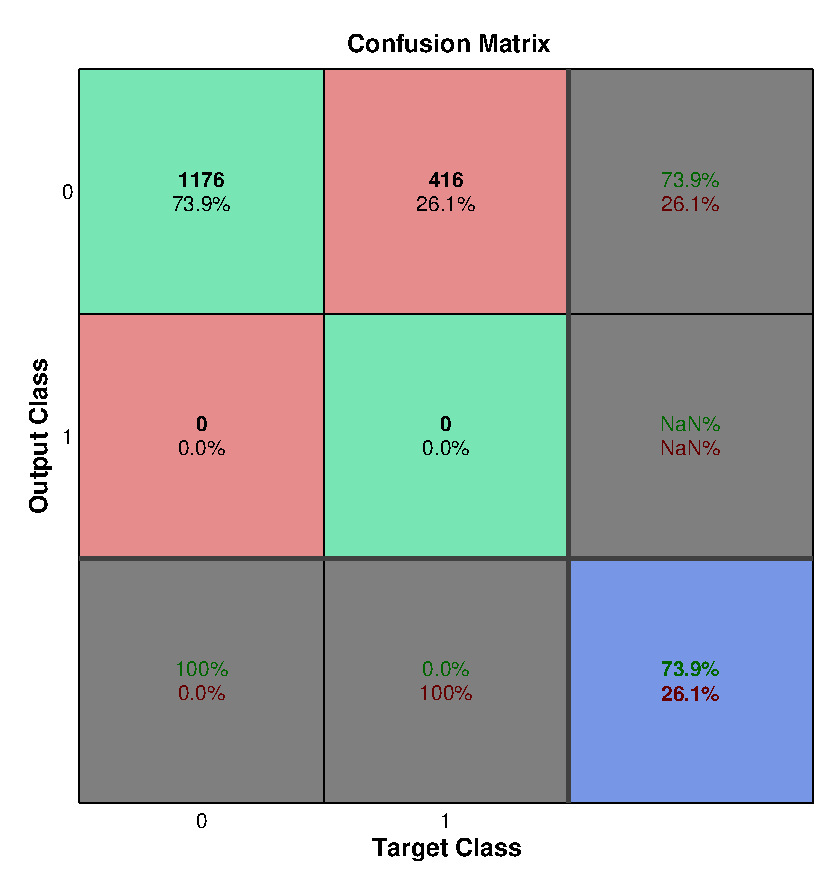
\includegraphics[width=0.45\linewidth]{Figures/CH5/NNBinaryOnset-hourly.eps}
	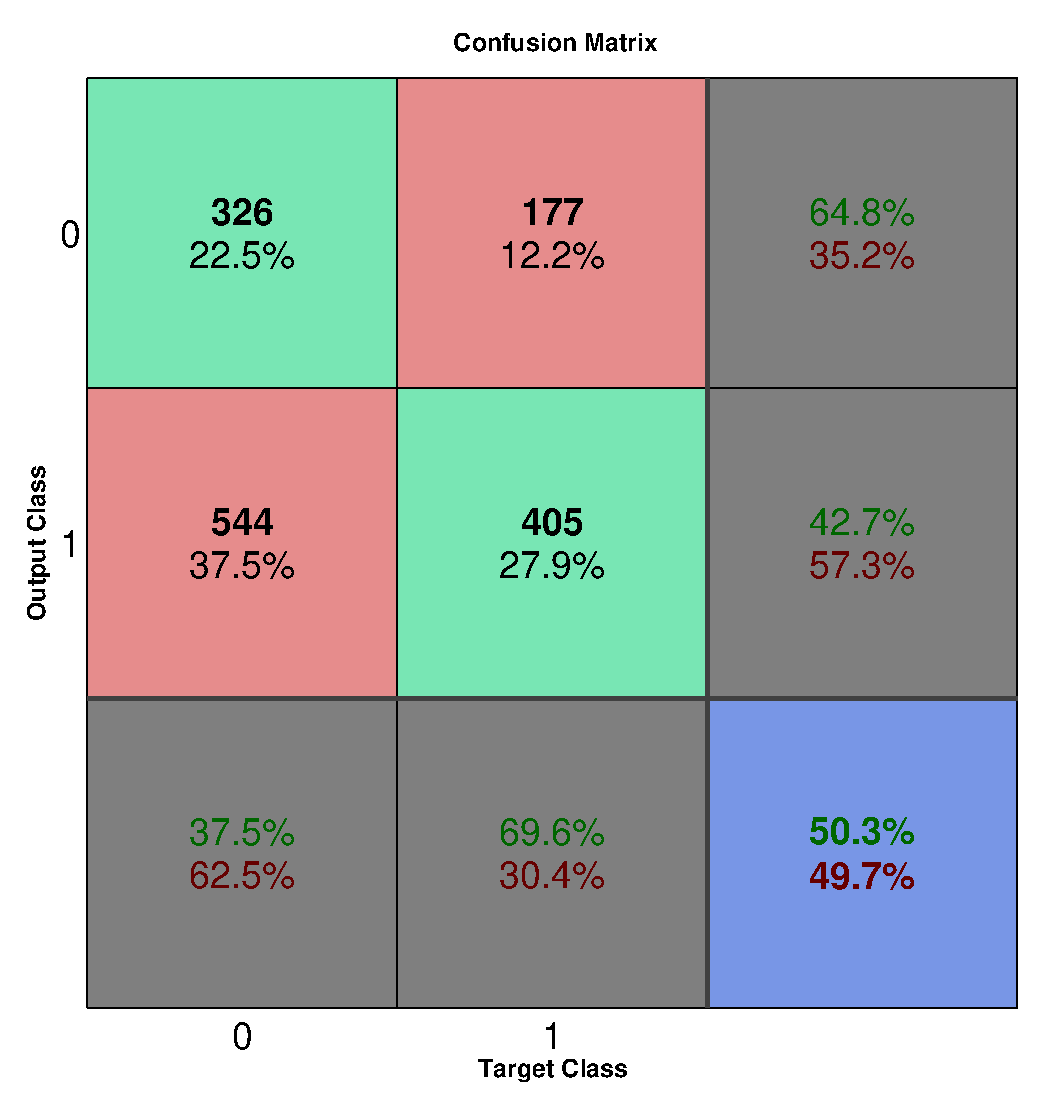
\includegraphics[width=0.45\linewidth]{Figures/CH5/NNBinaryOnset-daily.eps}
	\caption{Prediction confusion matrix for hourly (left) and daily (right) \req\ onset events using classification method}
	\label{fig:OnsetEvents}
\end{figure}

In an attempt to find out what conditions best lead to a correct prediction, histograms were made of the conditions associated with a correctly predicted onset vs those of an unpredicted onset. Figure \ref{fig:OnsetEventsHist} shows this for the four variables used.

\begin{figure}[htp!]
	\centering
	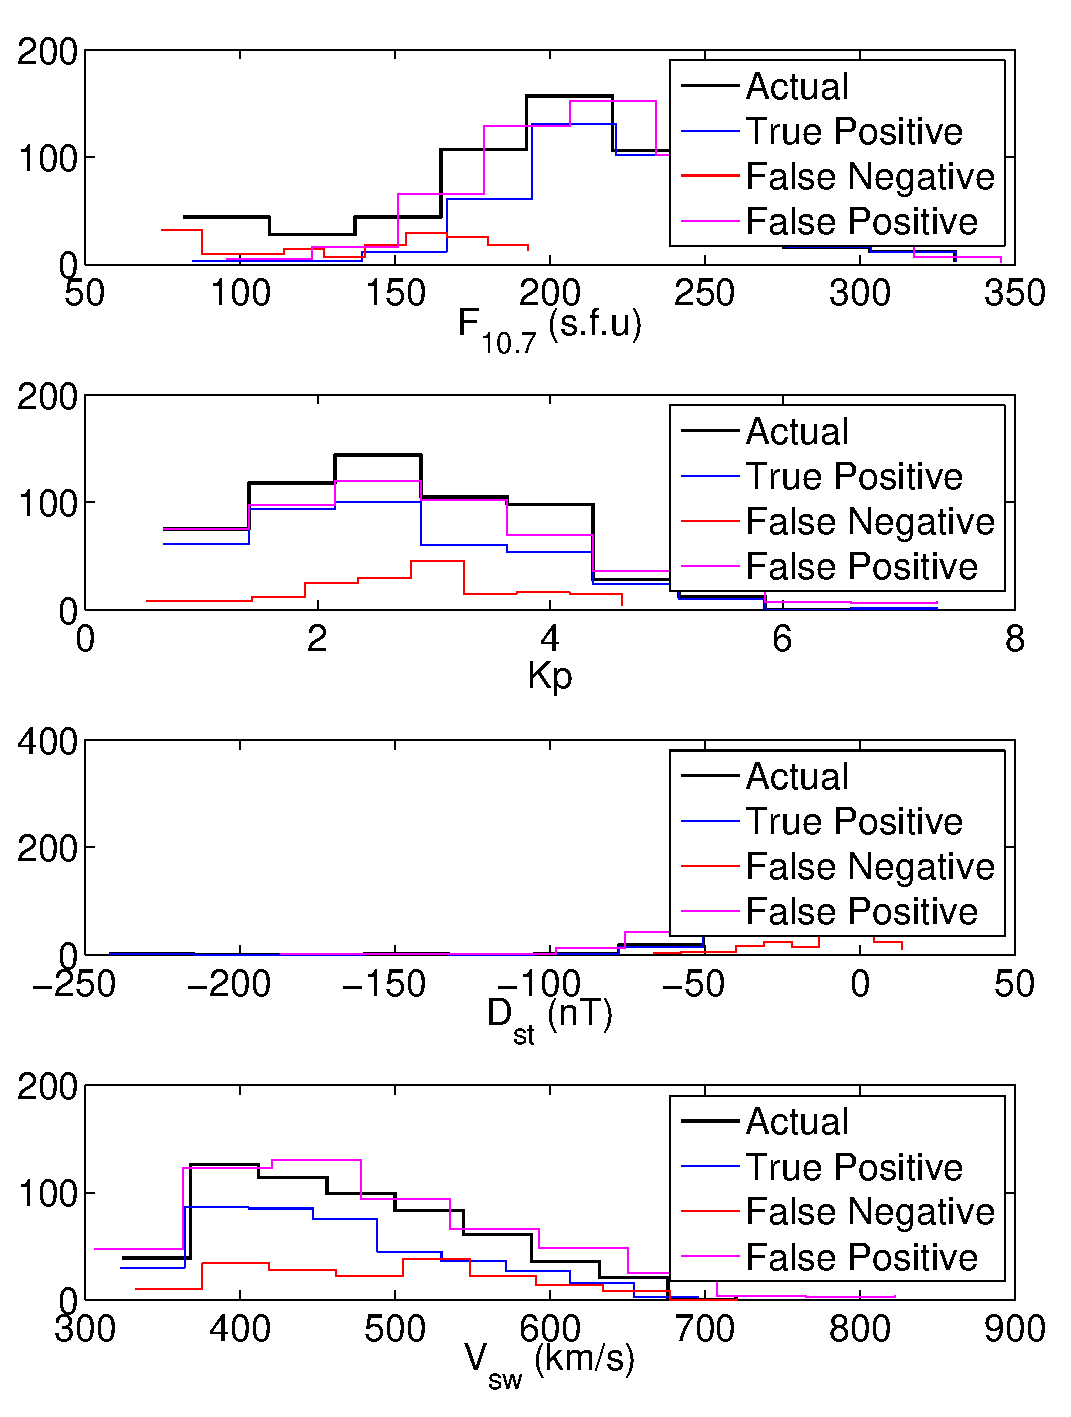
\includegraphics[width=0.85\linewidth]{Figures/CH5/NNBinaryOnset-daily-hist.eps}
	\caption{Histogram of onset conditions for \req\ events binned by correctness of prediction}
	\label{fig:OnsetEventsHist}
\end{figure}

It shows that the model tended to correctly predict onset more often when given a larger value of $F_{10.7}$, but that all other variables seemed to have a similar distribution between their correct and incorrect predictions. 

The next test was to add more obvious indicators of an event onset, such as the data being used to define an onset, and see if the model could pick that up. By adding \req\ as a factor in classifying \req\ events, the model unsurprisingly does very well, as shown in Figure \ref{fig:OnsetWithreq}.

\begin{figure}[htp!]
	\centering
	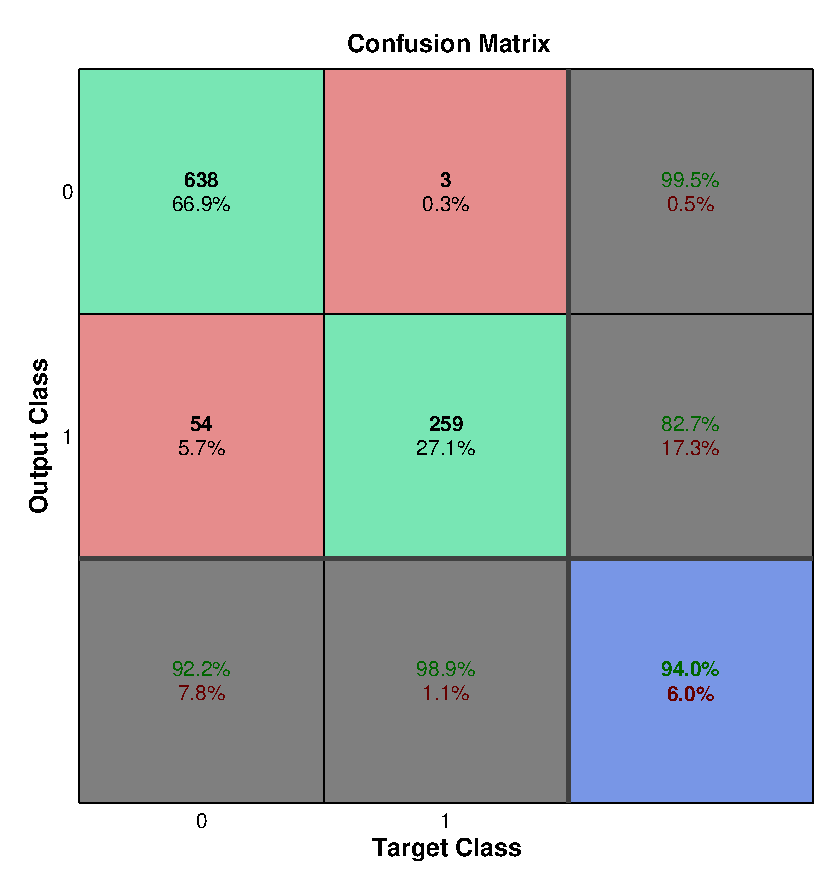
\includegraphics[width=0.45\linewidth]{Figures/CH5/NNBinaryOnset-hourly-withreq.eps}
	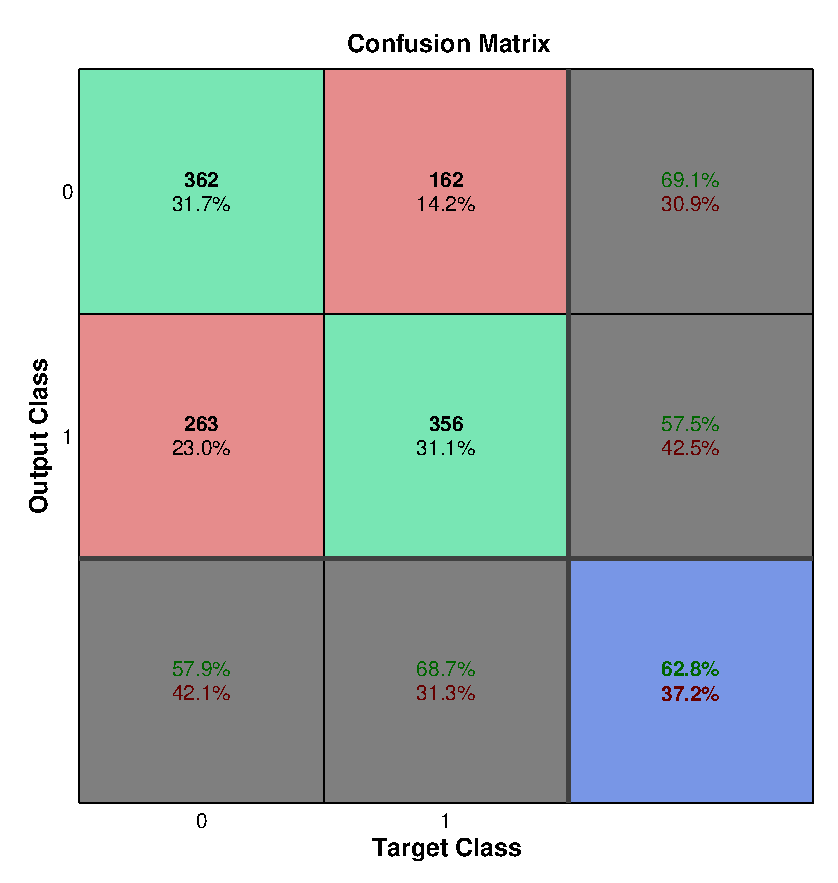
\includegraphics[width=0.45\linewidth]{Figures/CH5/NNBinaryOnset-daily-withreq.eps}
	\caption{Prediction confusion matrix for hourly (left) and daily (right) \req\ onset events, including \req\ as an input variable, and only looking at three hours before and including onset}
	\label{fig:OnsetWithreq}
\end{figure}

With a successful true positive classification rate of 81\% and 69\% for hourly and daily 4-hour models respectively, it can be said that including \req\ information makes the models effective for classifying event onset, but considering the event onsets are defined as a threshold of \req, perhaps it is more concerning that the models don't have a 100\% success rate. A histogram of these variables binned by true positive and false negative shows no particularly compelling trends, as seen in Figure \ref{fig:OnsetWithreq-hist}.


\begin{figure}[htp!]
	\centering
	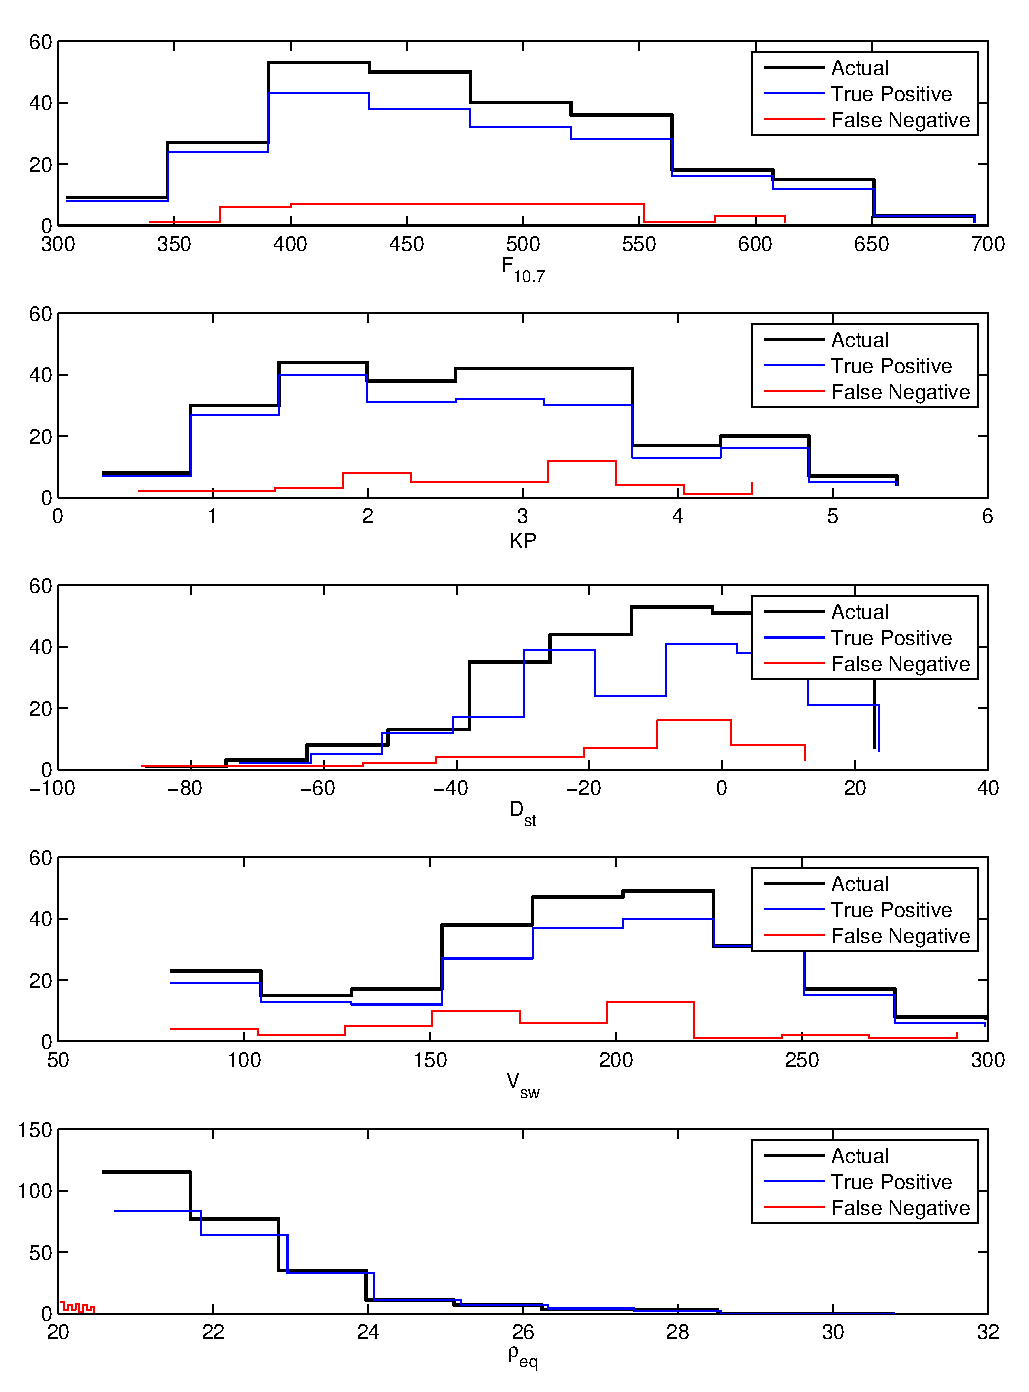
\includegraphics[width=1\linewidth]{Figures/CH5/NNBinaryOnset-hourly-withreq-hist.eps}
	\caption{Histogram of onset conditions for hourly \req\ events including \req\ as an input, binned by correctness of prediction}
	\label{fig:OnsetWithreq-hist}
\end{figure}

\subsection{Forecasting}

Using the full data set where each prediction was based on the current and previous three hours of inputs returned two models (daily and hourly) both of which predicted no onsets for \req\ events.



It is also interesting that including \req\ raises the detection rate for the daily model where all timesteps are included from 0\% to 10\%, as shown in Figure \ref{fig:OnsetFullWithreq}.

\begin{figure}[htp!]
	\centering
	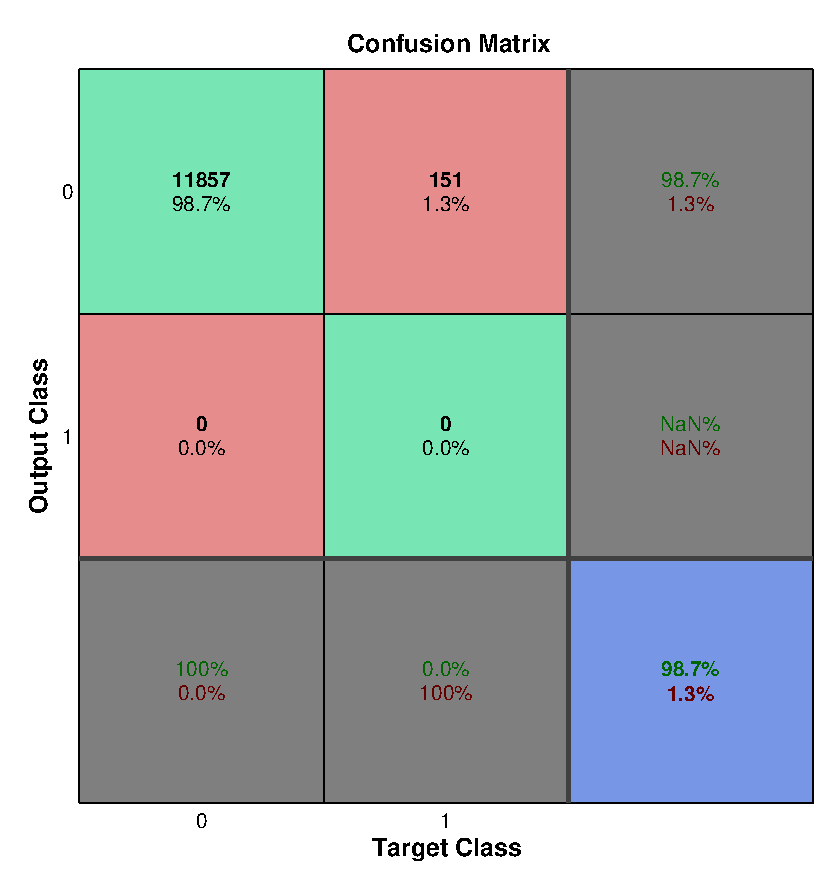
\includegraphics[width=0.45\linewidth]{Figures/CH5/NNBinaryOnset-full-hourly-withreq.eps}
	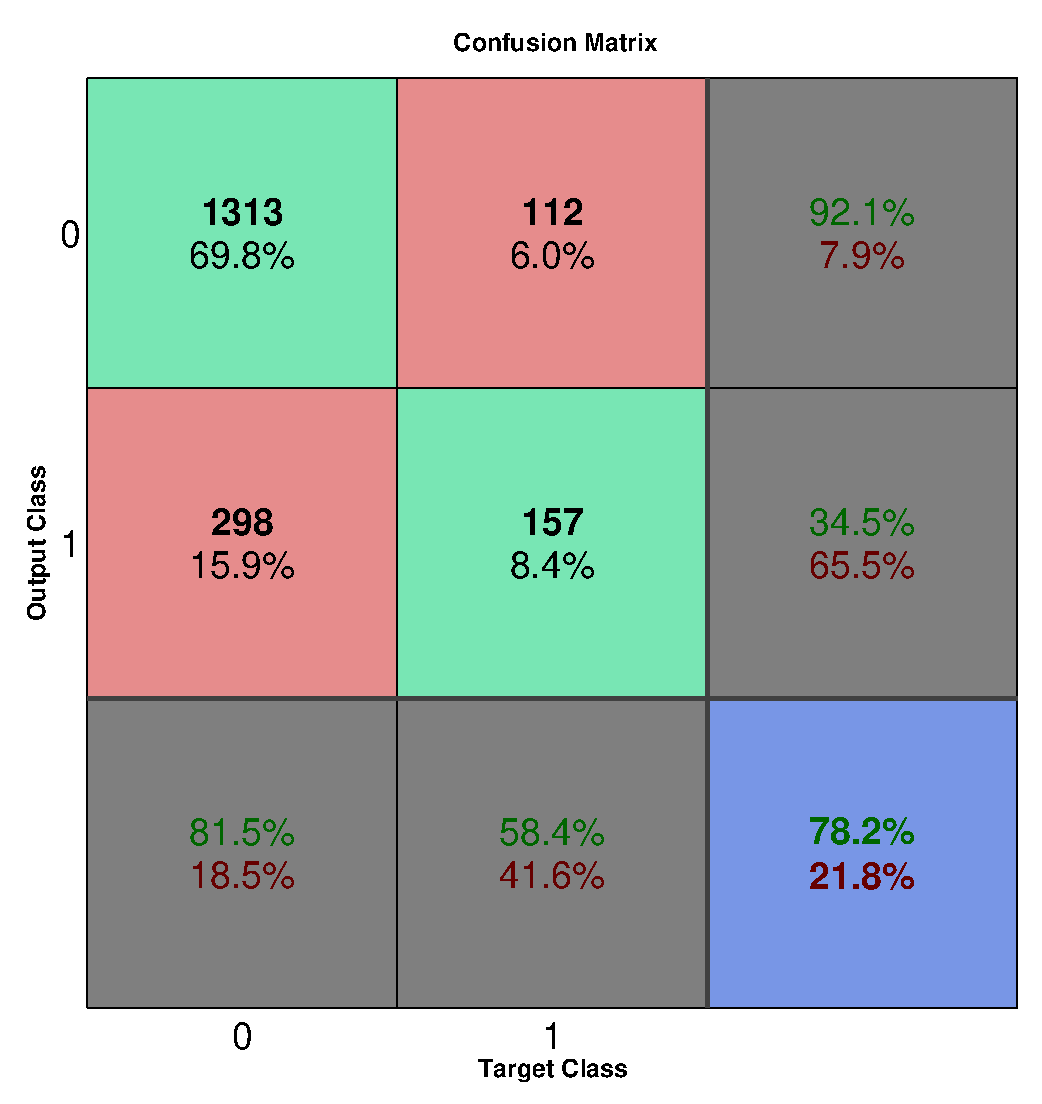
\includegraphics[width=0.45\linewidth]{Figures/CH5/NNBinaryOnset-full-daily-withreq.eps}
	\caption{Prediction confusion matrix for hourly (left) and daily (right) \req\ onset events, including \req\ as an input and using entire timeseries with a four hour sliding window}
	\label{fig:OnsetFullWithreq}
\end{figure}

This seems to suggest that work needs to be done to more heavily weight a "1" classification, so onsets are not drowned out by the far more numerous timesteps without an event onset.